\section*{Выполнение задания}
\addcontentsline{toc}{section}{Выполнение задания}

На рисунке \ref{fig:photo} представлена реализация алгоритма поиска подстроки в строке методом полного перебора.

\begin{figure}
	\centering
	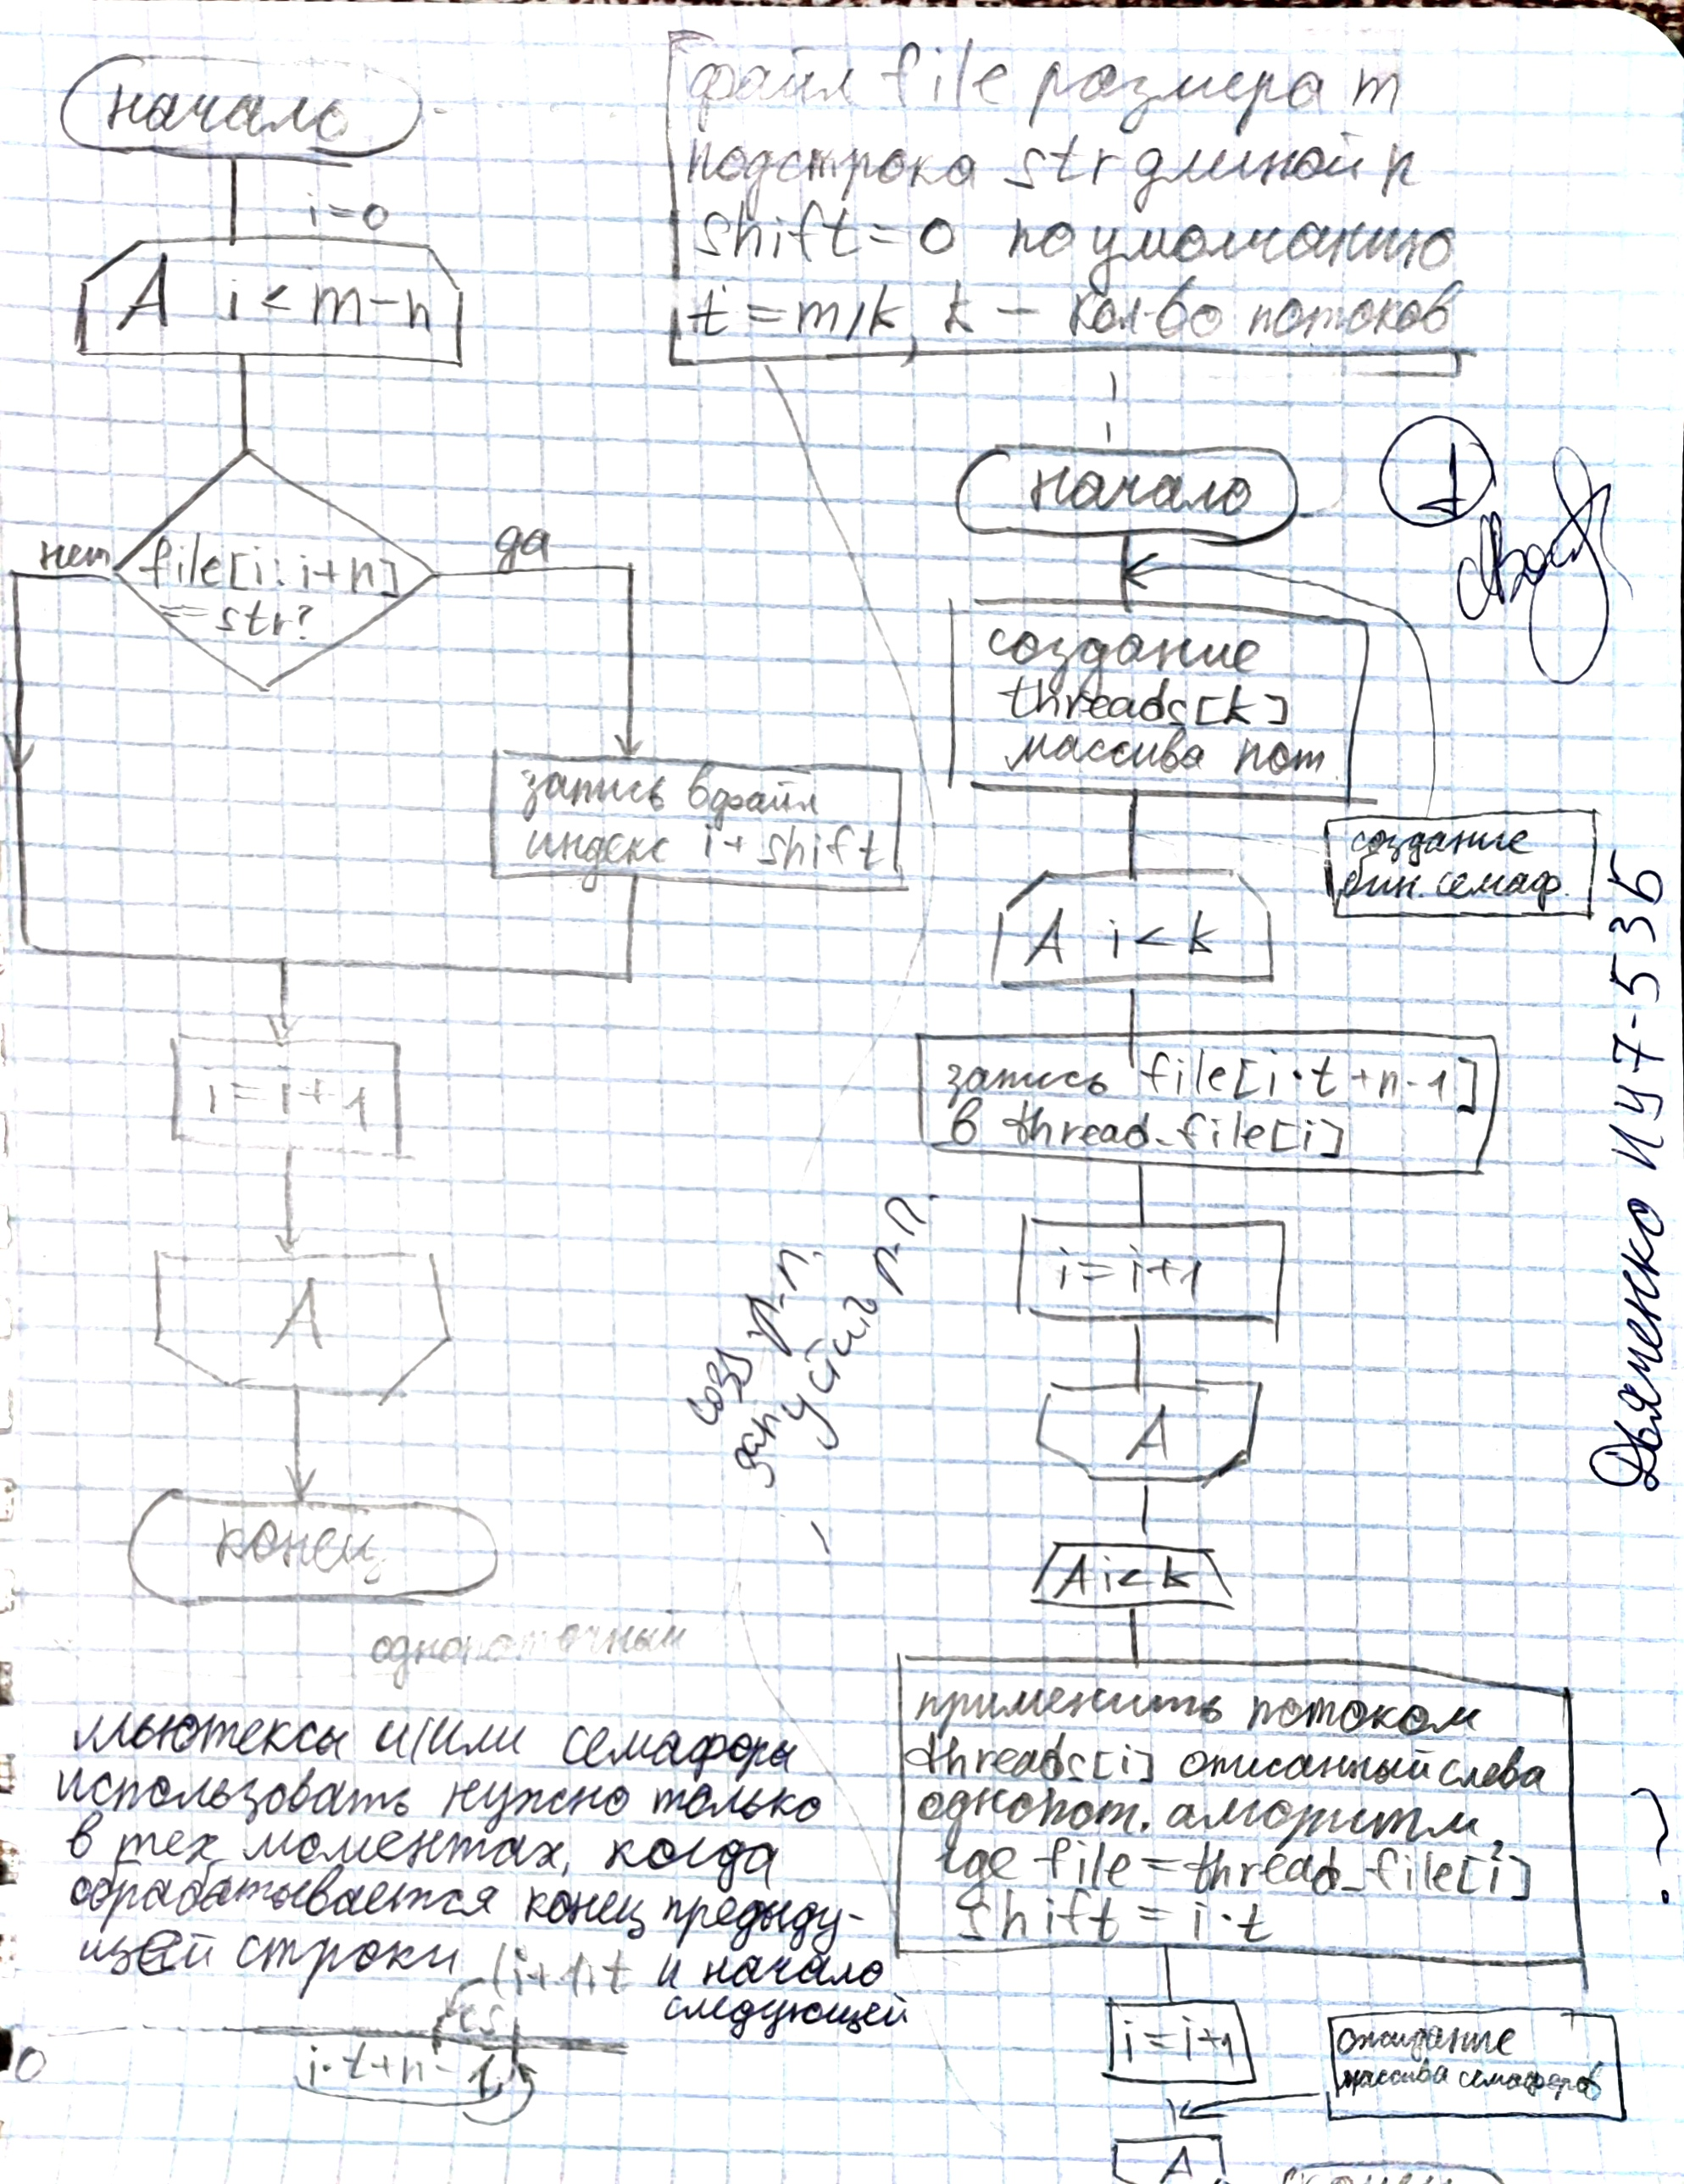
\includegraphics[width=0.7\linewidth]{task}
	\caption{Выполнение задания}
	\label{fig:photo}
\end{figure}

Входными данными являются файл и подстрока для поиска в этом файле.
Результат выводится в результирующий файл с указанием индекса символа, с которого
начинается искомая подстрока (нумерация начинается с 0).

Слева на рисунке расположен алгоритм поиска подстроки в строке.
Справа --- алгоритм главного потока, который инициализирует потоки и контролирует их завершение.

Снизу описан способ контроля доступа потоков к разделяемым ресурсам.